\documentclass[UTF8]{article}

\usepackage[UTF8]{ctex}

\usepackage{graphicx}
\usepackage{algorithm}
\usepackage{algorithmic}

\begin{document}

\title{Bisers: An efficient DHCPv6 address pool delimit solution}

\section{Abstract}

网络扫描是渗透测试的一个重要组成部分,然而IPv6网络因其庞大的地址空间而难以扫描。
针对使用DHCPv6管理的IPv6网络,探测DHCPv6服务器地址池的边界有助于缩小网络扫描的地址空间。
本文提出了一个DHCPv6定界方案:Bisers,通过若干次Ping和DHCPv6请求探测DHCPv6服务器的地址池的边界。
Bisers方案的优点是可以远程探测,探测速度快,准确率高,且对目前主流的DHCPv6实现普遍有效。
因此,Bisers方案可以有效地帮助扫描使用DHCPv6管理的IPv6网络。

\section{Introduction}

网络扫描是渗透测试的一个重要组成部分。
IPv4的地址空间只有32位,有限的地址空间决定了IPv4网络无法抵抗攻击者的网络扫描:
masscan等无状态扫描工具可以在几个小时内扫描整个IPv4网络,扫描一个子网可能只需要几分钟。
IPv6扩展了IPv4的地址空间到128位,庞大的地址空间使传统的网络扫描方法难以对其扫描。
随着IPv6的普及,寻找有效的IPv6网络扫描方法变得日益重要。

IPv6地址自动配置方式分为SLAAC(无状态地址自动配置)和DHCPv6(动态主机配置协议版本6)。
SLAAC虽然足以方便地配置网络,但是难于管理。
DHCPv6因其易于管理而被广泛使用在大型网络中。

本文提出了一个DHCPv6定界方案:Bisers(Binary Search \& Rebind \& Solicit),
可以快速准确地探测DHCPv6服务器的地址池的边界,帮助扫描使用DHCPv6管理的IPv6网络。

\subsection{Related Work}

本研究起始于Bergenholtz等人关于DHCPv6网络扫描的工作\cite{bergenholtz_finding_2019}:
他们提出了一个针对连续分配地址的DHCPv6服务器的定界算法:DeHCP。
该算法使用带窗口的二分搜索方法探测密集的地址空间的边界。
算法\ref{algoDeHCP}描述了DeHCP搜索下界的算法,搜索上界的算法类似。

\begin{algorithm}[H]
  \caption{DeHCP}
  \label{algoDeHCP}
  \renewcommand{\algorithmicrequire}{\textbf{Input:}}
  \renewcommand{\algorithmicensure}{\textbf{Output:}}
  \begin{algorithmic}[1]
    \REQUIRE Search range [a, b], Window size w
    \ENSURE Lower bound lb
    \STATE host <- (a + b) / 2
    \STATE if a >= b then return host
    \STATE if Ping(host) then return DeHCP(a, host-1, w)
    \STATE for h in host-w ... host+w:
    \STATE \ \ if Ping(h) then return DeHCP(a, h-1, w)
    \STATE return DeHCP(host+1, b, w)
  \end{algorithmic}
\end{algorithm}

该算法对于连续分配地址的DHCPv6服务器十分有效。
然而,我们发现为大型网络设计的DHCPv6服务器都使用更安全的随机地址分配方式。
因此,DeHCP的使用场景收到了更严格的限制。

\subsection{Main Work}

为弥补DeHCP的不足,我们提出了两个针对随机分配地址的DHCPv6服务器的定界算法:RDeHCP和SDeHCP。
前者基于DHCPv6协议的一个缺陷,可以实现精确定界但不总是有效。
后者基于数理统计估算出地址池的边界,精确率不如前者但普遍有效。
综合上述三种算法,我们提出了一个完善的DHCPv6定界方案:Bisers,针对不同特征的DHCPv6服务器选择不同的定界算法。
Bisers方案的探测过程大体如图\ref{figBisers}。

\begin{figure}[htbp]
  \caption{Bisers}
  \label{figBisers}
  \centering
  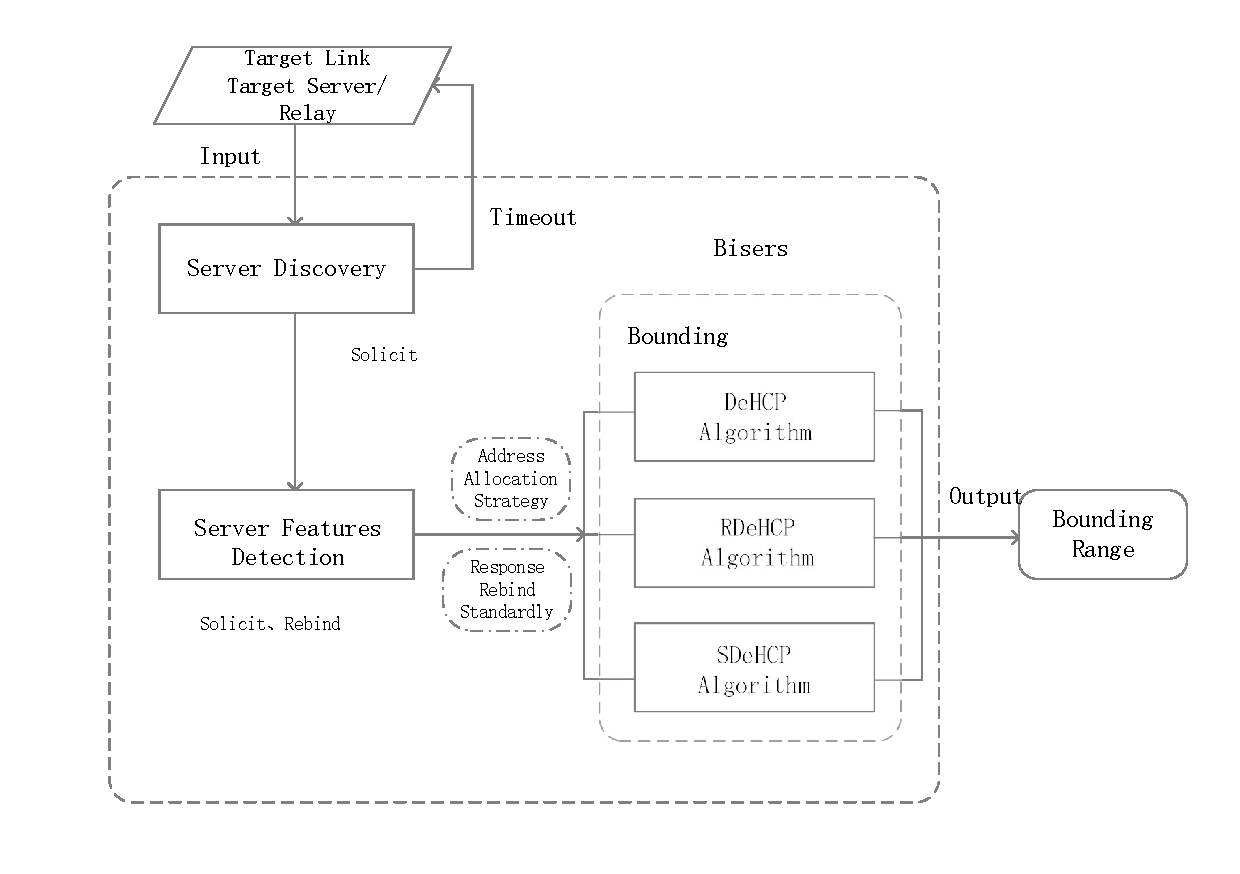
\includegraphics[scale=0.3]{bisers.pdf} \\
\end{figure}

我们给出了一个Bisers方案在Linux平台的参考实现\footnote{https://github.com/vhqr0/bisers}。

\section{Background}

DHCPv6是用来分配IPv6地址、前缀和其它网络参数的网络协议。
DHCPv6客户端向DHCPv6服务器租借并定期续租地址,
因此DHCPv6服务器可以轻易统计其管理的网络内的DHCPv6客户端的信息,相比于SLAAC更易于管理。

DHCPv6客户端与服务端的通信使用多播-单播的方式,在必要时用唯一标识DUID指定服务器。
客户端与服务端通过Solicit-Advertise-Request-Reply四步过程完成DHCPv6服务器发现与地址租借。
DHCPv6服务器借出的每一个地址都带有T1、T2值,分别表示续租超时时间和重新绑定超时时间,
当超过这些时间未及时续租地址时,分别用Renew-Reply过程和Rebind-Reply过程续租或重新绑定地址。

DHCPv6通过中继机制将多个链路的管理集中到一个DHCPv6服务器。
DHCPv6客户端的请求被封装到Relay报文中被中继层层转发至服务器,服务器再将响应封装到RelayReply报文中原路返回。
Relay报文中包含的链路地址字段决定服务器使用哪个地址池。

DHCPv6规范未规定DHCPv6服务器如何分配地址。
早期DHCPv6实现继承了DHCPv4的连续地址分配方式,但很快发现这种分配方式有严重的隐私问题。
因此,后来的DHCPv6实现大多采用随机地址分配方式。

\section{Bisers}

图\ref{figBisers}简要描述了Bisers方案的三个阶段:DHCPv6服务器发现阶段、DHCPv6服务器特征探测阶段和DHCPv6定界阶段。
下面我们对这三个阶段进行详细描述。

\subsection{DHCPv6 Server Discovery}

Bisers方案需要访问目标DHCPv6服务器,因此首先要根据扫描者与目标链路的位置关系确定要访问的DHCPv6服务器或中继及访问方式。
若要扫描的链路是本地链路,则可以直接访问本地DHCPv6服务器或中继(ff02::1:2)。
若要扫描的链路是远程链路,则需要通过中继的方式访问目标DHCPv6服务器。

通过中继的方式访问目标DHCPv6服务器的原理是模拟DHCPv6中继将DHCPv6请求封装到Relay报文,链路地址字段为目标链路地址,发送给目标服务器。
因此,在扫描前需要通过其它方法找到目标服务器或可以代理到此服务器的中继。
因为使用DHCPv6管理的站点的边缘路由器通常是代理到此站点DHCPv6服务器的中继,可以通过traceroute等工具找到这些中继。
如果扫描者与目标链路处于同一站点,则可以直接使用本地DHCPv6服务器或中继(ff02::1:2)。

在确定访问方式和要访问的服务器或中继后,通过Solicit请求快速探测目标服务器是否可以访问。
若可以访问则进行后续探测,否则探测失败,可以继续寻找其它服务器或中继。

\subsection{DHCPv6 Server Feature Detection}

本阶段探测DHCPv6服务器的地址分配方式是连续还是随机,以及是否支持使用Rebind探测地址池。
这些特征将决定使用何种定界算法探测该服务器的地址池的边界。

1. 地址分配方式:Bisers方案通过判断连续两次Solicit请求租借的地址是否连续判断服务器的地址分配方式是连续还是随机。
如果租借的地址A1和A2满足:|A1-A2|=1,则认为服务器的地址分配是连续地,否则认为是随机地。

2. 支持使用Rebind探测地址池:Bisers方案通过Rebind请求重新绑定已租借的地址附近的地址判断服务器是否支持使用Rebind探测地址池。
假设在服务器发现阶段租借到的地址为A,则尝试重新绑定地址A+1和A-1,如果有一个成功则认为服务器支持使用Rebind探测地址池。

\subsection{DHCPv6 Delimit}

Bisers方案通过前阶段探测到的特征决定使用何种定界算法。
这些算法都可以通过若干次DHCPv6请求和Ping请求探测出DHCPv6服务器的地址池的边界。
针对连续分配地址的DHCPv6服务器使用DeHCP算法。
针对随机分配地址的DHCPv6服务器,我们提出两个定界算法:RDeHCP和SDeHCP。
关于两个算法的描述如下:

1. RDeHCP

RDeHCP算法基于DHCPv6协议的一个缺陷:当DHCPv6服务器收到Rebind报文时,服务器应根据重新绑定的地址是否符合其地址分配策略给出响应。
我们简单假设DHCPv6服务器根据重新绑定的地址是否在其地址池中给出响应,当我们重新绑定地址A时,有三种情况:
A不在地址池中,A在地址池中但已被分配和A在地址池中且未被分配。前两种情况将绑定失败,后一种情况将绑定成功。
因为在庞大的地址池中取少数几个地址与服务器已分配的地址产生碰撞的概率很低,我们可以直接忽略第二种情况,当绑定失败时认为A不在地址池中。

算法\ref{algoRDeHCP}描述了RDeHCP搜索下界的算法,搜索上界的算法类似。
RDeHCP通过类似DeHCP的二分搜索方法探测服务器的地址池边界。

\begin{algorithm}[H]
  \caption{RDeHCP}
  \label{algoRDeHCP}
  \renewcommand{\algorithmicrequire}{\textbf{Input:}}
  \renewcommand{\algorithmicensure}{\textbf{Output:}}
  \begin{algorithmic}[1]
    \REQUIRE Search range [a, b]
    \ENSURE Lower bound lb
    \STATE host <- (a + b) / 2
    \STATE if a >= b then return host
    \STATE if Rebind(host)
    \STATE \ \ then return RDeHCP(a, host-1)
    \STATE \ \ else return RDeHCP(host+1, b)
  \end{algorithmic}
\end{algorithm}

2. SDeHCP

RDeHCP算法可以实现精确定界,但并非所有实现的地址池都可以使用Rebind探测。
对于这些实现,我们提出一个更通用的定界算法:SDeHCP算法。

算法\ref{algoSDeHCP}描述了SDeHCP算法:通过n次Solicit请求地址,记录请求到的地址的最大值与最小值a',b'。
假设服务器随机分配地址,可以计算出地址池的边界的期望[a-$\delta$,b+$\delta$],其中$\delta$=$\frac{b'-a'}{n-1}$。

\begin{algorithm}[H]
  \caption{SDeHCP}
  \label{algoSDeHCP}
  \renewcommand{\algorithmicrequire}{\textbf{Input:}}
  \renewcommand{\algorithmicensure}{\textbf{Output:}}
  \begin{algorithmic}[1]
    \REQUIRE Solicit times n
    \ENSURE Pool boundary [a', b']
    \STATE host <- Solicit()
    \STATE minhost <- host, maxhost <- host
    \STATE dotimes n:
    \STATE \ \ host <- Solicit()
    \STATE \ \ minhost <- min(host, minhost)
    \STATE \ \ maxhost <- max(host, maxhost)
    \STATE delta <- (maxhost - minhost) / n
    \STATE return [minhost - delta, maxhost + delta]
  \end{algorithmic}
\end{algorithm}

\section{Experiment and Analysis}

为了评估Bisers方案,我们先进行仿真实验,再对几个主流的DHCPv6实现进行实际测试。
我们引入准确率作为衡量一个定界算法效果的指标:
假设真实的地址池为[a, b],定界算法得到的地址池为[a', b'],定义准确率为$1-\frac{|a'-a| + |b'-b|}{b-a}$。

\subsection{Simulation for Bisers}

为了初步评估Bisers方案的准确率与寻找合适的参数,我们通过仿真实验模拟真实环境,测试三个算法在不同环境、不同参数下的准确率。
模拟环境的DHCPv6服务器地址池大小为48位,网络规模为1000,在测试DeHCP时连续分配地址,在测试其它算法时随机分配地址。
模拟环境在测试DeHCP和RDeHCP时将分别模拟30\%、50\%、70\%的离线主机比例,SDeHCP与离线主机比例无关,不再分别测试。
针对DeHCP,我们将分别测试窗口大小为1、2、3、4时在不同环境下的定界准确率。
针对SDeHCP,我们将分别测试请求次数为32、64、128、256时的定界准确率。
仿真实验的结果将用于选择合适的参数进行后续的实际测试。
实验结果见表\ref{tabDeHCP}、\ref{tabRDeHCP}、\ref{tabSDeHCP}。
通过实验结果可以看到取DeHCP窗口大小为3,SDeHCP请求次数为128时已有很好的效果,三个算法的定界准确率都接近99\%。

\begin{table}[htbp]
  \caption{DeHCP}
  \label{tabDeHCP}
  \centering
  \begin{tabular}{|c|c|c|c|}
    \hline
    Windows size \textbackslash Offline host ratio & 30\% & 50\% & 70\% \\
    \hline
    1 & 99.8\% & 91.16\% & 53\% \\
    2 & 99.8\% & 93.96\% & 83.22\% \\
    3 & 99.8\% & 98.54\% & 94.86\% \\
    4 & 99.8\% & 99.7\% & 98.7\% \\
    \hline
  \end{tabular}
\end{table}

\begin{table}[htbp]
  \caption{RDeHCP}
  \label{tabRDeHCP}
  \centering
  \begin{tabular}{|c|c|c|c|}
    \hline
    Offline host ratio & 30\% & 50\% & 70\% \\
    \hline
    Accuracy & 100\% & 100\% & 100\% \\
    \hline
  \end{tabular}
\end{table}

\begin{table}[htbp]
  \caption{SDeHCP}
  \label{tabSDeHCP}
  \centering
  \begin{tabular}{|c|c|c|c|c|}
    \hline
    Solicit times & 32 & 64 & 128 & 256 \\
    \hline
    Accuracy & 96.34\% & 97.93\% & 98.97\% & 99.49\% \\
    \hline
  \end{tabular}
\end{table}

\subsection{Practical Testing for Bisers}

我们选择几个主流的DHCPv6实现进行实际测试,分别是:
TPLink路由器\footnote{TL-XDR1860}、Cisco路由器\footnote{IOS 7200}、Openwrt\footnote{19.07}、
ISC DHCP Server\footnote{4.4.1}和Windows DHCP Server\footnote{Windows Server 2016},
涵盖了家用路由器、商用路由器、最常见的软路由及软件实现。
针对每一个实现,我们先统计其一些基本特征,包括是否支持通过中继远程访问、地址分配方式、默认的地址池大小等,
这些特征将影响Bisers方案的表现。然后再测试Bisers方案对该实现的准确率:
先配置DHCPv6服务器,如果没有默认的DHCPv6配置可用,则手动配置大小为24位的地址池。
在测试之前,先租借1000个地址,再用Bisers方案定界并统计准确率。

实际测试的结果见表\ref{tabDHCPv6Server}。
通过测试结果可以看到Bisers方案对这些DHCPv6实现普遍有效。
除了TPLink路由器使用连续地址分配,不支持子网及地址池配置,无法通过中继访问,
其它DHCPv6服务端实现都采用随机地址分配,子网与地址池配置,且支持通过中继远程访问。
在使用随机地址分配的服务端实现中,Openwrt强制使用8位的地址池,易于扫描;
Windows DHCP Server使用64位的地址池,难以扫描;
Cisco路由器和ISC DHCP Server扫描的难易程度取决于手动配置的地址池的大小。

\begin{table}[htbp]
  \caption{Mainstream DHCPv6 Server Test Results}
  \label{tabDHCPv6Server}
  \centering
  \begin{tabular}{|c|c|c|c|c|c|}
    \hline
    DHCPv6 Server & Cisco & TPLink & Openwrt & Windows & ISC \\
    \hline
    Remote access & Yes & No & Yes & Yes & Yes \\
    Address assignment type & Random & Linear & Random & Random & Random \\
    Rebind based probe & No & No & No & No & Yes \\
    Default pool size & Manual & N/A & 8 & 64 & Manual \\
    Accuracy & 99.2\% & 100\% & 96.9\% & 99.1\% & 100\% \\
    \hline
  \end{tabular}
\end{table}

\subsection{安全建议}

我们从两方面提出防止DHCPv6探测的建议:
首先,一个站点的网关应该通过防火墙规则过滤掉所有进出站点的DHCPv6报文;
其次,一个站点的所有边缘路由器应对DHCPv6协议的报文进行特殊处理。

RFC7610定义了DHCPv6 Shield,一个在2层网络设备上对DHCPv6报文的转发作出限制的技术,旨在防范流氓DHCPv6服务器。
该技术在2层设备在部署前需要指定可信端口,在转发报文时需要判断该报文是否是DHCPv6服务端报文,仅转发来自可信端口的DHCPv6服务端报文。
我们为DHCPv6 Shield提出了一个隐私扩展来防止DHCPv6被动扫描和非法访问DHCPv6服务器:
2层设备在转发报文时应判断一个报文是否是DHCPv6服务端报文、客户端报文或中继报文。
2层设备应丢弃所有中继报文和来自不可信端口的服务端报文,且只向可信端口转发服务端报文。

该隐私扩展可以杜绝远程Bisers探测及本地链路被动扫描,但无法防止Bisers本地探测。
DHCPv6服务器应使用随机地址分配和大地址池来防止主动扫描。

\subsection{总结及进一步工作}

本文提出了一个DHCPv6定界方案:Bisers。该方案基于DHCPv6协议,通过若干次Ping和DHCPv6请求探测DHCPv6服务器的地址池边界。
通过仿真实验及在目前主流的DHCPv6服务器下实际测试,我们验证了该方案的速度与准确率:
Bisers方案对本文选择的几个测试对象都有效,且只需要数百个DHCPv6报文或Ping报文就可以在几秒内完成定界,定界准确率超过95\%。
因此,在实际扫描过程中先尝试定位DHCPv6服务器或中继并通过Bisers方案缩小扫描的地址空间不会浪费太多时间,而且可能取得较好的效果。

对本研究的进一步工作的方向可以放在远程定位DHCPv6服务器或中继的方法,
以及如何利用通过Bisers方案可以得到的DHCPv6服务器的附加信息,如T1值,是否支持LeaseQuery,是否支持RapindCommit等。

\bibliography{cites}

\end{document}